%##############################################################################
\chapter{Analyse des Regelkreises}
%##############################################################################
%
Um einen Regelkreis auslegen zu können, benötigt es zunächst Methoden, um dessen Verhalten zu beschreiben. Diese Analysemethoden werden verwendet, um den Regelkreis zu quantifizieren und somit später für die jeweilige Regelstrecke zu entwerfen.
%
\section{Modell des Standardregelkreis \cite{MSF05,Lunze10}}
\label{sec:standardregelkreis}
%
In den letzten Kapiteln wurden die Grundglieder des Regelkreises erläutert und die grundsätzlichen dynamischen Modelle eingeführt. Dies bildet die Grundlagen, um nun die Eigenschaften des Regelkreises einzuführen. Der Standardregelkreis im Laplacebereich, kann mit folgenden Komponenten dargestellt werden, siehe Abbildung~\ref{fig:standardRegelkr}.
%
\begin{figure}[h!]
	\centering
	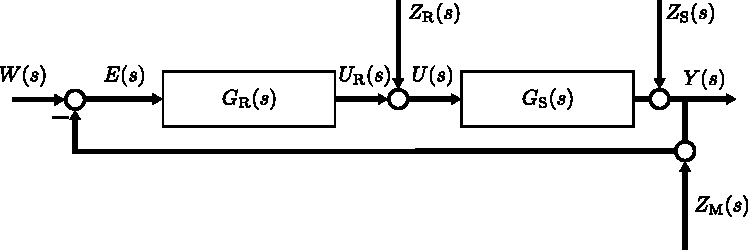
\includegraphics[width=0.95\linewidth]{Abbildungen/Systemanalyse/PDF/Standardregelkreis.pdf}
	\caption{Abbildung der Komponenten im Standardregelkreis}
	\label{fig:standardRegelkr}
\end{figure}
%
Die Gesamtübertragungsfunktion des Regelkreises ergibt sich aus der Summe der einzelnen beteiligten Signale zu 
%
\begin{equation*}
\begin{aligned}
	%
	Y(s)=G_{\text{W}}(s)W(s)+G_{\text{ZR}}(s)Z_{\text{R}}(s)+G_{\text{ZS}}(s)Z_{\text{S}}(s)+G_{\text{ZM}}(s)Z_{\text{M}}(s)
	%
\end{aligned}
\end{equation*}  
%
Hierbei sind die beteiligten Übertragungsfunktionen
%
\begin{itemize}
	\item $G_{\text{R}}(s)$ die Übertragungsfunktion des Reglers.
	\item $G_{\text{S}}(s)$ die Übertragungsfunktion der Regelstrecke.
	\item $G_{\text{W}}(s)$ die Führungsübertragungsfunktion.
	\item $G_{\text{ZR}}(s)$ die Störübertragungsfunktion für Störsignale am Streckeneingang.
	\item $G_{\text{ZS}}(s)$ die Störübertragungsfunktion für Störsignale am Streckenausgang.
	\item $G_{\text{ZM}}(s)$ die Störübertragungsfunktion für Störsignale im Messsignal der Regelgröße.
\end{itemize}  
%
Zentraler Bestandteil der genannten Übertragungsfunktionen ist das Verhalten des offenen Kreises. Dieses ist definiert als Hintereinanderschaltung des Reglers und der Strecke ohne eine Rückführung.
%
\begin{equation*}
\begin{aligned}
	%
	G_{0}(s)=G_{\text{R}}(s)G_{\text{S}}(s)\\
	%
	\end{aligned}
\end{equation*} 
%
Verfolgt man die Signalpfade der Regelung aus Abbildung~\ref{fig:standardRegelkr}, so lassen sich durch Umformen die bereits genannten Übertragungsfunktionen bilden 	
%
\begin{equation*}
	\begin{aligned}
		%
		G_{\text{W}}(s)=\frac{G_{0}(s)}{1+G_{0}(s)}\\
		%
		G_{\text{ZR}}(s)=\frac{G_{\text{S}}(s)}{1+G_{0}(s)}\\
		%
		G_{\text{ZS}}(s)=\frac{1}{1+G_{0}(s)}\\
		%
		G_{\text{ZM}}(s)=\frac{1}{1+G_{0}(s)}
		%
	\end{aligned}
\end{equation*}  
%
Die Störübertragungsfunktionen werden meist in eine gemeinsame Darstellung $G_{\text{Z}}(s)=\frac{1}{1+G_{0}(s)}$ überführt, da ja durch die Linearität die Wirkungen der Störungen, immer auch vor oder nach der Strecke verschoben werden können, wie in Abbildung~\ref{fig:standardRegelkreinfach} dargestellt.
Hiermit ergibt sich die Gesamtübertragungsfunktion des geschlossenen Regelkreises zu
%
\begin{equation*}
\begin{aligned}
%
Y(s)=\underbrace{\frac{G_{0}(s)}{1+G_{0}(s)}}_{G_{\text{W}}(s)}W(s)+\underbrace{\frac{1}{1+G_{0}(s)}}_{G_{\text{Z}}(s)}Z(s)
%
\end{aligned}
\end{equation*}   
%
\begin{figure}[h!]
	\centering
	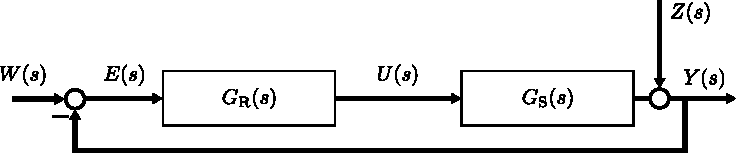
\includegraphics[width=0.95\linewidth]{Abbildungen/Systemanalyse/PDF/StandardregelkreisEinfach.pdf}
	\caption{Vereinfachte Darstellung der Komponenten im Standardregelkreis}
	\label{fig:standardRegelkreinfach}
\end{figure}
%
%
Die Forderungen an den Regelkreis kann nun auf die einzelnen Übertragungsfunktion abgebildet werden. Die Führungssprungantwort soll $G_{\text{W}}(s\rightarrow 0)=h_{\text{W}}(t \rightarrow\infty)\approx 1$ sein, so dass gilt $Y(s\rightarrow 0)=W(s\rightarrow 0)$, während die Störübertragungsfunktionen $G_{\text{ZR}}(s\rightarrow 0)\approx 0$, $G_{\text{ZS}}(s\rightarrow 0)\approx 0$, $G_{\text{ZM}}(s\rightarrow 0)\approx 0$ sein sollen, so dass Störungen des Regelkreises abklingen.
Nehmen wir nun weiter an, das der Regelkreis eingeschwungen ist, und sämtliche Störgrößen abgeklungen sind. Des Weiteren soll $G_{\text{R}}(s)=K_{\text{P}}$ sein und die Regelstrecke durch ihre stationäre Verstärkung beschrieben werden $G_{\text{S}}(s\rightarrow 0)=K_{\text{S}}$. Die Führungsübertragungsfunktion ergibt sich somit zu
%
\begin{equation*}
\begin{aligned}
	%
	\lim\limits_{t\rightarrow\infty}h_{\text{W}}(t)=\lim\limits_{s\rightarrow 0}sH_{\text{W}}(s)=\lim\limits_{s\rightarrow 0}G_{\text{W}}(s)&=\frac{K_{\text{P}}K_{\text{S}}}{1+K_{\text{P}}K_{\text{S}}}\\
	%
	&=\frac{1}{\frac{1}{K_{\text{P}}K_{\text{S}}}+1}
	%
\end{aligned}
\end{equation*}    
%
Die Forderung nach Sollwertfolge $G_{\text{W}}(s\rightarrow 0)\approx 1$ kann hier nur erfüllt werden, wenn $K_{\text{P}}\rightarrow \infty$. \underline{Allgemein gilt:} falls die Regelstrecke proportionales Verhalten besitzt, so benötigt der Regler einen integralen Anteil, um eine bleibende Regelabweichung zu kompensieren. Dies lässt sich in gleicher Form auch für die Regeldifferenz aufstellen, um das Störverhalten zu analysieren 
%
\begin{equation*}
\begin{aligned}
%
E(s)=W(s)-\left(Z(s)+G_{0}(s)E(s)\right)\\
%
E(s)=\frac{1}{1+G_{0}(s)}W(s)-\frac{1}{1+G_{0}(s)}Z(s)
%
\end{aligned}
\end{equation*}  
%
Über den Endwertsatz lässt sich hieraus eine Bedingung für die stationäre Genauigkeit ableiten.
%
\begin{equation*}
\begin{aligned}
%
e_{\infty}&=\lim\limits_{t\rightarrow\infty}e(t)=\lim\limits_{s\rightarrow 0}s E(s)\\
%
e_{\infty}&=\lim\limits_{s\rightarrow 0}s\frac{1}{1+G_{0}(s)}W(s)-\lim\limits_{s\rightarrow 0}s\frac{1}{1+G_{0}(s)}Z(s)
%
\end{aligned}
\end{equation*}  
%
Wird nun angenommen, dass es sich um sprungförmige Stör- und Führungssignale handelt, so kann die Gleichung vereinfacht werden zu
%
\begin{equation*}
\begin{aligned}
%
e_{\infty}&=\lim\limits_{s\rightarrow 0}\frac{1}{1+G_{0}(s)}\left(w_{0}-z_{0}\right)\\
%
&=\frac{1}{1+\lim\limits_{s\rightarrow 0}G_{0}(s)}\left(w_{0}-z_{0}\right)
%
\end{aligned}
\end{equation*}  
%
Aus dieser Gleichung wird ersichtlich, dass der Grenzwert $\lim\limits_{s\rightarrow 0}G_{0}(s)$, darüber entscheidet, ob die stationäre Regeldifferenz $e_{\infty}$ verschwindet. Allgemein gesprochen muss die Übertragungsfunktion des offenen Regelkreises in der Form 
%
\begin{equation*}
\begin{aligned}
	%
	G_{0}(s)=\tilde{G}_{0}(s)\frac{1}{s}
	%
\end{aligned}
\end{equation*} 
%
dargestellt werden können. Ist dies der Fall so hat der Regelkreis für sprungförmige Stör- und Führungssignale keine bleibende Regelabweichung und ist somit stationär genau. Diese Beobachtung lässt sich auch auf weitere Signaltypen erweitern. Zusammengefasst ergibt sich 
%
\begin{itemize}
	%
	\item Bei impulsförmigen Stör- und Führungssignalen $(w_{0}\delta(t),z_{0}\delta(t))$ muss der offene Regelkreis nur stabil sein.
	%
	\item Bei sprungförmigen Stör- und Führungssignalen $(w_{0}\sigma(t),z_{0}\sigma(t))$ muss der offene Regelkreis ein I-Glied enthalten.
	%
	\item Bei rampenförmigen Stör- und Führungssignalen $(w_{0}t,z_{0}t)$ muss der offene Regelkreis ein I$_{2}$-Glied enthalten.
	%
\end{itemize}
%
\section{Analyse der Stabilität des geschlossenen Regelkreises}
\label{sec:stabilitaet}
%
\subsection{Technische Beispiele für Stabilität}
%
Die Stabilität technischer Systeme beschreibt die Eigenschaft auf eine bestimmte, jedoch beschränkte, Systemgröße mit einem beschränkten Ausgangssignal zu reagieren. 

Der Stabilitätsbegriff soll im Folgenden Anhand einer Reihenschaltung aus Kondensator und elektrischen Widerstand veranschaulicht werden. In Abbildung~\ref{fig:rcglied} ist die Schaltung mit einer Spannungsquelle, einem Schalter, so wie den konzentrierten Elementen Kondensator und Widerstand dargestellt.
%
\begin{figure}[h]
	\centering
	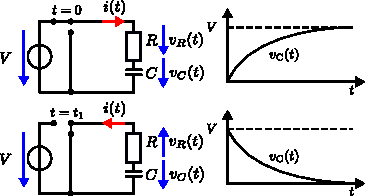
\includegraphics[width=0.7\linewidth]{Abbildungen/Modellbildung/PDF/RCglied.pdf}
	\caption{RC-Glied als Beispiel eines Zustands und E/A-Stabilen Systems}
	\label{fig:rcglied}
\end{figure}
%
Zum Zeitpunkt $t=0$ wird der Schalter auf die Spannungsquelle umgeschaltet und der Kondensator auf die Spannung $V$ aufgeladen. Die sprungförmige Anregung durch die Spannungsquelle $V$ kann als beschränktes Eingangssignal interpretiert werden. Der Ausgang des Systems, hier mit $v_{\text{c}}(t)$ gewählt, strebt gegen diesen endlichen Wert, das System ist somit E/A-Stabil.
%
Wird nun zum Zeitpunkt $t=t_{1}$ der Schalter umgelegt (siehe Abbildung~\ref{fig:rcglied} unten) und der Kondensator über den Widerstand entladen, klingt die Spannung am Kondensator ab. Die Kondensatorspannung zum Zeitpunkt $t=t_{1}$ stellt den Anfangswert des nicht angeregten Systems dar. Somit kann für dieses Beispiel auch die asymptotische Stabilität gewährleistet werden.
%
\subsubsection{Beispiele für instabile Systeme}
%
Ein häufig verwendetes Beispiel für instabile Systeme ist das inverse Pendel. Es handelt sich hierbei um ein mathematisches Pendel (aus dem Physikunterricht), welches an der horizontalen Achse gespiegelt wurde. Es besitzt somit nicht mehr den Gleichgewichtspunkt $\varphi=0$, wie in Abbildung~\ref{fig:inversespendel}, links dargestellt. Stattdessen ist das Pendel für diesen Arbeitspunkt nun instabil und fällt von diesem Punkt aus in eine Richtung um. Es gibt die Möglichkeit das inverse Pendel durch einen Regler zu stabilisieren und somit für technische Anwendungen verwendbar zu machen. Beispiele hierfür sind Roboter auf zwei Rädern \cite{Lunze10} oder eine schwebende Kugel im Magnetfeld \cite{Dastych13}.
%
\begin{figure}[h]
	\centering
	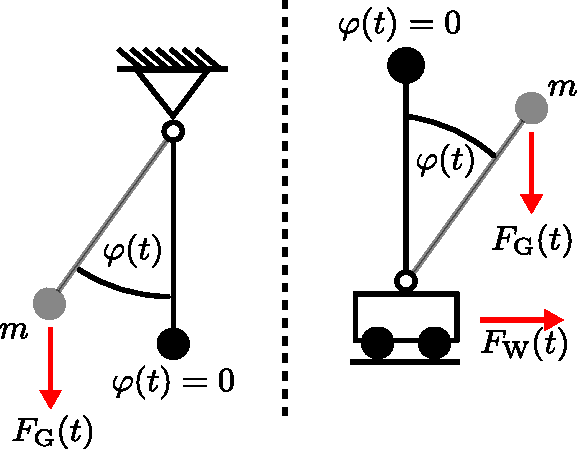
\includegraphics[width=0.5\linewidth]{Abbildungen/Systemanalyse/PDF/InversesPendel.pdf}
	\caption{Mathematisches und mögliche Ausprägung als inverses Pendel}
	\label{fig:inversespendel}
\end{figure}  
%
\begin{python}{}{}
	\begin{itemize}
		\item \textit{Animation: inverses Pendel mit freier Bewegung (Darstellung der Instabilität)}
	\end{itemize}
\end{python}
%
\subsection{Stabilitätsprüfung anhand der Übertragungsfunktion \cite{Lunze10}}
%
Die Stabilität des geschlossenen Regelkreises basiert auf der Analyse der E/A-Stabilität. Das E/A-Verhalten ist durch die Gesamtübertragungsfunktion
%
\begin{equation*}
\begin{aligned}
%
Y(s)=\underbrace{\frac{G_{0}(s)}{1+G_{0}(s)}}_{G_{\text{W}}(s)}W(s)+\underbrace{\frac{1}{1+G_{0}(s)}}_{G_{\text{Z}}(s)}Z(s)
%
\end{aligned}
\end{equation*}   
%
gegeben, wie bereits erwähnt ist in dieser Vorlesung asymptotische Stabilität und E/A-Stabilität gleichwertig. Da beide Übertragungsfunktionen das selbe Nennerpolynom besitzen, reicht es, eine charakteristische Gleichung der Form
%
\begin{equation*}
\begin{aligned}
%
F_{0}(s)=1+G_{0}(s)\\
%
\end{aligned}
\end{equation*}
%
zu betrachten. Nur diese Polstellen dazu bei, ob das System stabil oder instabil ist. Zerlegen wir diese Gleichung in ihre weiteren Bestandteile, so erhalten wir eine Darstellung in Zähler- $Z_{0}(s)$ und Nennerpolynom $N_{0}(s)$ der Übertragungsfunktion $G_{0}(s)$
%
\begin{equation*}
\begin{aligned}
%
F_{0}(s)=1+\frac{Z_{0}(s)}{N_{0}(s)}=\frac{N_{0}(s)+Z_{0}(s)}{N_{0}(s)}.\\
%
\end{aligned}
\end{equation*}
%
In $N_{0}(s)+Z_{0}(s)$ sind die Pole des geschlossenen Regelkreises enthalten, weshalb zur Stabilitätsberechnung diese charakteristische Gleichung zu Null gesetzt wird und deren Wurzeln bestimmt werden.
%
\begin{equation*}
\begin{aligned}
%
N_{0}(s)+Z_{0}(s)&=0\\
%
\overline{a}_{n}\overline{s}^{n}+\overline{a}_{n-1}\overline{s}^{n-1}+\overline{a}_{n-2}\overline{s}^{n-2}+\dots+\overline{a}_{0}&=0
%
\end{aligned}
\end{equation*}
%
Die Lösungen $\overline{s}_{\text{P},1},\overline{s}_{\text{P},2},...,\overline{s}_{\text{P},n}$ dieses Polynoms bestimmen, ob der Regelkreis stabil oder instabil ist. Der Regelkreis ist genau dann E/A-stabil, wenn alle Pole einen negativen Realteil besitzen.
%
\begin{equation*}
\begin{aligned}
%
\Re\{\overline{s}_{i}\}<0, \,\, \forall i \in \{1,...,n\}
%
\end{aligned}
\end{equation*}
%
Diese notwendige und hinreichende Bedingung kann beispielsweise mit dem Hurwitz-Kriterium überprüft werden.
%
\begin{Aufgaben}{}{}
	\begin{itemize}
		\item \textit{Stabilitätsüberprüfung mittels Hurwitz-Kriterium}
	\end{itemize}
\end{Aufgaben}
%
\textbf{Zusammenfassung der Stabilitätsanalyse}:
\begin{itemize}
	\item Berechnung der Wurzeln der charakteristischen Gleichung.
	\item Falls hohe Ordnung entweder Computer gestützte Verfahren oder Routh-Hurwitz-Kriterium.
	\item Alle Realteile der Wurzeln, der charakteristischen Gleichung aus $N_{0}(s)+Z_{0}(s)$ müssen negativ sein.
\end{itemize} 
%
%\subsection{Der Frequenzgang des offenen Regelkreises} 
%%
%\subsubsection{Die Ortskurve des offenen Regelkreises}
%%
%Der Frequenzgang kann wie bereits im vorherigen Kapitel~\ref{chap:Modellbildung} vorgestellt, im Bodediagramm, oder auch Frequenzkennliniendiagramm genannt, dargestellt werden. Eine weitere Form der Darstellung ist die Ortskurve. Diese stellt den Amplituden- und Phasengang des Frequenzgangs in der komplexen Ebene mit $\omega$ als Parameter dar. Dieser Zusammenhang ist in Abbildung~\ref{fig:Ortskurve} dargestellt.
%%
%\begin{figure}[h!]
%	\centering
%	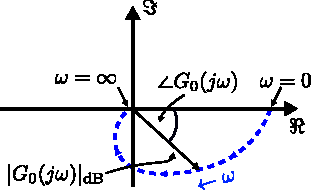
\includegraphics[width=0.45\linewidth]{Abbildungen/Systemanalyse/PDF/Ortskurve.pdf}
%	\caption{Ortskurve des offenen Regelkreises}
%	\label{fig:Ortskurve}
%\end{figure}
%%
%Aus dieser Darstellung ist ersichtlich, dass sich die Grenzwertsätze im Frequenzbereich auch in graphischer Form darstellen lassen. Nehmen wir das IT$_{1}$-Glied als Beispiel, so erhalten wir für den Frequenzgang
%%
%\begin{equation*}
%\begin{aligned}
%%
%G_{0}(j\omega)&=\frac{1}{j\omega T_{\text{I}}\left(j \omega T_{1}+1\right)}\\
%%
%&=\frac{1}{\left(-\omega^{2}T_{\text{I}}T_{1}+j\omega T_{\text{I}}\right)}\cdot\frac{\left(-\omega^{2}T_{\text{I}}T_{1}-j\omega T_{\text{I}}\right)}{\left(-\omega^{2}T_{\text{I}}T_{1}-j\omega T_{\text{I}}\right)}\\
%%
%&=\frac{-\omega T_{1}-j}{\omega T_{\text{I}}\left(\omega^{2}T^{2}_{1}+1\right)}\\
%%
%&=\frac{-T_{1}}{T_{\text{I}}\left(\omega^{2}T^{2}_{1}+1\right)}-j\frac{1}{\omega T_{\text{I}}\left(\omega^{2}T^{2}_{1}+1\right)}\\
%%
%\end{aligned}
%\end{equation*} 
%%
%Hieraus lassen sich nun der Anfangs- und Endwert aus der Grenzwertbetrachtung
%%
%\begin{equation*}
%\begin{aligned}
%%
%\lim\limits_{\omega\rightarrow \infty}G_{0}(j\omega)&=0\\
%%
%\lim\limits_{\omega\rightarrow 0}\Re\{G_{0}(j\omega)\}&=-\frac{T_{1}}{T_{\text{I}}}\\
%%
%\lim\limits_{\omega\rightarrow 0}\Im\{G_{0}(j\omega)\}&=-\infty.
%%
%\end{aligned}
%\end{equation*} 
%%
%ermitteln und nachfolgend die Ortskurve zeichnen (siehe Abbildung~\ref{fig:OrtskurveIT1}).
%%
%\begin{figure}[h!]
%	\centering
%	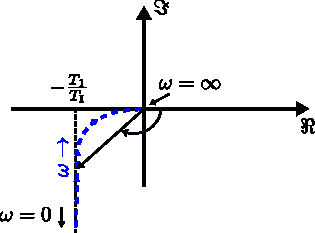
\includegraphics[width=0.50\linewidth]{Abbildungen/Systemanalyse/PDF/OrtskurveIT1.pdf}
%	\caption{Ortskurve des IT$_{1}$-Gliedes}
%	\label{fig:OrtskurveIT1}
%\end{figure}
%%
%Es soll hier zudem erwähnt werden, dass der Verlauf der Amplitude und der Phase von $\omega=0$ bis $\omega=\infty$ auch durch die bekannten Verfahren der Frequenzkennlinie berechnet werden kann. 
%%
%\subsubsection{Die Frequenzkennlinien des offenen Regelkreises}
%%
%Die Darstellung in der Ortskurve ist nicht die einzige Möglichkeit, um das Verhalten des Regelkreises zu analysieren. Im vorherigen Kapitel~\ref{chap:Modellbildung} haben wir bereits im Bodediagramm eine weitere Darstellungsform kennengelernt. Allgemein wird diese auch als Frequenzkennlinie (FKL) bezeichnet. Im nachfolgenden wird der Frequenzgang des offenen Regelkreises in die Form
%%
%\begin{equation*}
%\begin{aligned}
%%
%G_{0}(j\omega)=k \underbrace{\cdot \frac{1}{(j\omega)^{q}}}_{\text{I-Glieder}} \cdot \underbrace{\frac{\prod_{i=1}\left(j \omega T_{i}+1\right)}{\prod_{\nu=1}\left(j \omega T_{\nu}+1\right)}}_{\text{PT}_{1}~\text{-Glieder}} 
%%
%\cdot\underbrace{\frac{\prod_{k=1}\left(\left(\frac{j \omega}{\omega_{0 k}}\right)^{2}+\frac{j \omega}{\omega_{0 k}} 2 d_{k}+1\right)}{\prod_{\mu=1}\left(\left(\frac{j \omega}{\omega_{0 \mu}}\right)^{2}+\frac{j \omega}{\omega_{0 \mu}} 2 d_{\mu}+1\right)}}_{\text{PT}_{2}~\text{-Glieder}} 
%%
%\cdot \underbrace{e^{-T_{t}j\omega}}_{\text{Totzeit-Glied}} 
%%
%\end{aligned}
%\end{equation*}  
%%
%gebracht. Durch die Überlagerung dieser Grundglieder lässt sich der Frequenzgang $G_{0}(j\omega)$ möglichst genau darstellen. Bedingung hierfür ist jedoch das:
%%
%\begin{itemize}
%	\item $0<d_{k},d_{\nu}<1$: gedämpft aber schwingungsfähig.
%	\item $\omega_{0k},\omega_{0\mu},T_{i},T_{\nu},T_{t}>0$: Kausalitätsbedingung.
%	\item $k>0$: Gegenkopplungsbedingung.
%	\item $q \le 2$: Bedingung für Stabilitätsnachweis über vereinfachtes Nyquistkriterium. 
%\end{itemize}
%%
%Somit ergibt sich, dass $G_{0}(j\omega)$ sich aus den Frequenzgängen der Grundglieder und deren Inversen zusammensetzt. Die Rechenregeln hierfür lauten:
%%
%\begin{equation*}
%\begin{aligned}
%%
%\quad\quad &G(j\omega)=|G(j\omega)|e^{j\varphi},\,\varphi=\angle G(j\omega)\\
%%
%\end{aligned}
%\end{equation*}
%%
%Die Inversionsregel ergibt sich zu:
%%
%\begin{equation*}
%\begin{aligned}
%%
%\quad\quad  &G^{-1}(j\omega)=\frac{1}{|G(j\omega)|}e^{-j\varphi}\\
%%
%&|G^{-1}(j\omega)|=\frac{1}{|G(j\omega)|}.\\
%%
%\end{aligned}
%\end{equation*}
%%
%Was sich im Amplituden und Phasengang zu:
%%
%\begin{equation*}
%\begin{aligned}
%%
%&|G^{-1}(j\omega)|_{\text{dB}}=20\lg\left(\frac{1}{|G(j\omega)|}\right)=-20\lg\left(|G(j\omega)|\right)\\
%%
%&\angle G^{-1}(j\omega) = - \angle G(j\omega)
%%
%\end{aligned}
%\end{equation*}
%%
%ergibt. Es ist ersichtlich, dass die Inversion zu einer Spiegelung der FKL an der Null-Linie führt ($0_{\text{dB}}$ bzw. $0^{\circ}$).\\ Die Multiplikationsregel hingegen ergibt sich zu:
%%
%\begin{equation*}
%\begin{aligned}
%%
%\quad\quad &G(j\omega)=G_{1}(j\omega)\cdot G_{2}(j\omega) \cdot\ldots\cdot G_{n}(j\omega)\\
%%
%&G(j\omega)=|G_{1}(j\omega)|e^{j\varphi_{1}}\cdot|G_{1}(j\omega)|e^{j\varphi_{1}}\cdot \ldots \cdot |G_{n}(j\omega)|e^{j\varphi_{n}}\\
%%
%&G(j\omega)=\left(|G_{1}(j\omega)|\cdot|G_{2}(j\omega)|\cdot\ldots\cdot|G_{n}(j\omega)\right)e^{j\left(\varphi_{1}+\varphi_{2}+\ldots+\varphi_{n}\right)}\\
%%
%\end{aligned}
%\end{equation*}
%%
%Was sich im wiederum im Amplituden- bzw. Phasengang zu:
%%
%\begin{equation*}
%\begin{aligned}
%%
%|G(j\omega)|_{\text{dB}}&=20\lg\left(|G_{1}(j\omega)|\cdot|G_{2}(j\omega)|\cdot\ldots\cdot|G_{n}(j\omega)\right)\\
%%
%&=20\lg\left(|G_{1}(j\omega)|\right)+20\lg\left(|G_{2}(j\omega)|\right)+\ldots+20\lg\left(|G_{n}(j\omega)|\right)\\
%%
%\angle G(j\omega) &=\angle G_{1}(j\omega)+\angle G_{2}(j\omega)+\ldots+\angle G_{n}(j\omega)
%%
%\end{aligned}
%\end{equation*}
%%
%ergibt. Das bedeutet, dass eine Multiplikation der Frequenzgänge eine Addition in der FKL zur Folge hat. \underline{Hinweis:} Eine Multiplikation ist gleichbedeutend mit der Hintereinanderschaltung einzelner Übertragungsglieder im Wirkschaltplan.
%
\subsection{Stabilitätsprüfung anhand des Frequenzgangs}
\subsubsection{Das vereinfachte Nyquist-Kriterium}
%
Anhand dieses Kriteriums kann durch die Analyse des offenen Regelkreises auf die Stabilität des geschlossenen Regelkreises geschlussfolgert werden. Das vereinfachte Nyquist-Kriterium ist ein Spezialfall des allgemeinen Nyquist Kriteriums und ist nur auf stabile Strecken $G_{\text{S}}(s)$ und resultierende kausale $G_{0}(s)$ mit maximal zwei enthaltenen I-Gliedern anwendbar. Der offene Regelkreis muss sich folgendermaßen darstellen lassen: 
%
\begin{equation*}
\begin{aligned}
%
&G_{0}(s)=\frac{1}{s^{2}}\cdot\tilde{G}_{0}(s).\\
%
\end{aligned}
\end{equation*}
%
Mit $\tilde{G}_{0}(s)$ dem Teil der offenen Kette die kein I-Glied enthält. Da die meisten offenen Regelkreise jedoch diese Anforderung erfüllen, ist dieses zur Betrachtung der Stabilität ausreichend. Das Nyquist-Kriterium nutzt die Ortskurve, um die Gegenkopplungsbedingung der Rückführung im geschlossenen Kreis zu prüfen. Die Gegenkopplungsbedingung besagt vereinfacht, dass das Rückführungssignal der Regelgröße $y(t)$ und der Sollwert bzw. die Führungsgröße $w(t)$ ein am Additionspunkt stationär entgegengesetztes Vorzeichen besitzen müssen. Dies ist aus dem Standardregelkreis (Abbildung~\ref{fig:standardRegelkreinfach}) ersichtlich, da gilt $E(s)=W(s)-Y(s)$ oder im Zeitbereich $e(t)=w(t)-y(t)$.\\\\
%
Die Gegenkopplungsbeziehung kann somit als eine Phasenverschiebung der beiden Signale von $180^{\circ}$ zueinander interpretiert werden. Eine weitere Phasenverschiebung führt zu einer Mitkopplung, wenn die Kreisverstärkung $|G_{0}(j\omega_{180^{\circ}})|=K_{0}$ größer als eins ist. Hierdurch wird der Regelkreise instabil. In der Ortskurve lässt sich dieser Zusammenhang an der Umschlingung des Punktes $-1+j0$ analysieren. Eine Ortskurve, welche diesen Punkt umschlingt, ist in Abbildung~\ref{fig:LinkeHandRegel} dargestellt.
%
\begin{figure}[h!]
	\centering
	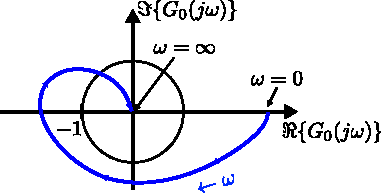
\includegraphics[width=0.55\linewidth]{Abbildungen/Systemanalyse/PDF/LinkeHandRegel.pdf}
	\caption{Grafische Darstellung des vereinfachten Nyquist-Kriteriums für einen instabilen Regelkreis}
	\label{fig:LinkeHandRegel}
\end{figure}\\
%
\begin{itemize}
%
\item \underline{\textbf{Merke:}} Ein Regelkreis ist
genau dann stabil, wenn der Punkt $-1+j0$ im Bereich $0<\omega<\infty$ von der Ortskurve der offenen Kette $G_{0}(j\omega)$ weder umschlossen noch durchlaufen wird \cite{Foellinger94}
%
\end{itemize}
%
%
\subsubsection{Erweiterung auf Regelkreise mit Totzeit}
%
Enthält die offene Kette ein Totzeit-Glied $G_{0}(s)=\frac{1}{s^{2}}\tilde{G}_{0}(s)\cdot e^{-T_{t}s}$, so kann das Kriterium immer noch angewendet werden. Dies ist eine Stärke des vereinfachten Nyquist-Kriteriums, denn für diesen Fall wäre das Hurwitz-Kriterium nicht mehr anwendbar. Es sollte berücksichtigt werden, dass durch das Totzeit-Glied lediglich die Phase verändert wird, nicht jedoch die Amplitude des Frequenzgangs. Im folgenden sind vier Beispiele für Ortskurven und deren zugehörigen qualitativen Übertragungsfunktionen dargestellt (siehe Abbildung~\ref{fig:Beispiele}). 
%
\begin{figure}[h!]
	\centering
	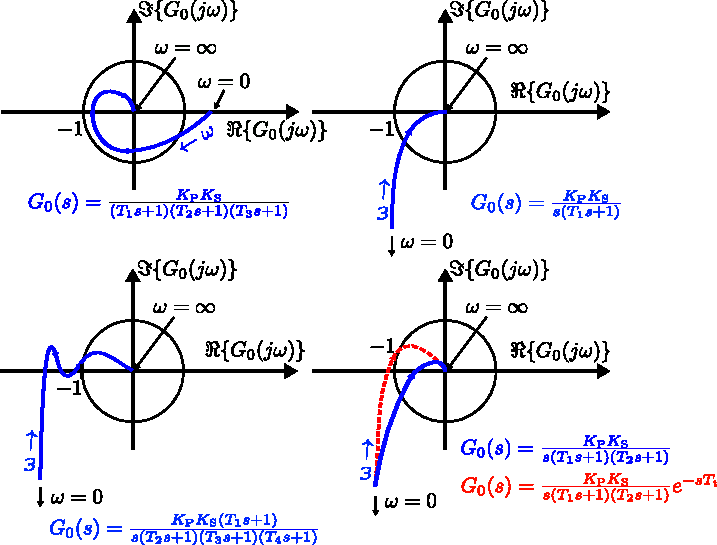
\includegraphics[width=.95\linewidth]{Abbildungen/Systemanalyse/PDF/Ortskurven_Beispiele.pdf}
	\caption{Beispielhafte Ortskurven für stabile Systeme (oben) und instabile Systeme (unten). Das IT$_{2}T_{\text{t}}$-System im unteren rechten Bereich, wird durch eine Totzeit instabil}
	\label{fig:Beispiele}
\end{figure}
%
\newpage
%
\textbf{Zusammenfassung der Stabilitätsanalyse}:
\begin{itemize}
	\item Nur möglich für offene Regelkreise die aus einer stabilen Strecke mit maximal zwei I-Gliedern entstehen 
	\item Totzeitglieder können berücksichtigt werden.
	\item Umschlingung des Punktes $-1+j0$ durch die Ortskurve bestimmt die Stabilität des geschlossenen Kreises.
	\item Für die Auswertung der Ortskurve sind immer rechnergestützte Verfahren notwendig.
\end{itemize} 
%
\subsubsection{Das Phasenrandkriterium}
%
Eine weitere anschauliche Darstellung kann durch den Vergleich von Ortskurve und Frequenzkennlinie erfolgen. Da die Frequenzkennlinie ja genutzt werden kann, um die Ortskurve zu skizzieren, enthält sie alle Informationen für eine Untersuchung der Stabilität. Sie ist jedoch gegenüber der Ortskurve wesentlich einfacher zeichnerisch zu konstruieren. 
%
\begin{figure}[h!]
	\centering
	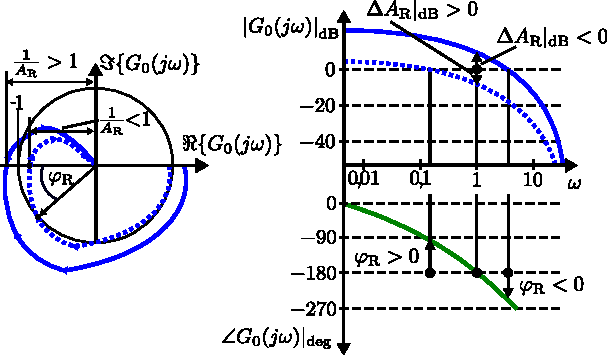
\includegraphics[width=.8\linewidth]{Abbildungen/Systemanalyse/PDF/Phasenrand.pdf}
	\caption{Phasenrandkriterium und Zusammenhand zwischen Ortskurve und Frequenzkennlinie}
	\label{fig:Phasenrand}
\end{figure}
%
Im folgenden ist die Frequenzkennlinie und die zugehörige Ortskurve nebeneinander dargestellt (siehe Abbildung~\ref{fig:Phasenrand}). Durch eine Änderung der Reglerverstärkung wird in der Frequenzkennlinie der Amplitudengang nach oben oder unten verschoben (rechter Teil der Abbildung~\ref{fig:Phasenrand}; gestrichelte blaue Linie), ohne das sich der Phasengang ändert. Dies ergibt sich aus der Tatsache, dass die Reglerverstärkung lediglich die Ortskurve skaliert (linker Teil der Abbildung~\ref{fig:Phasenrand}). Um die Stabilität des geschlossenen Regelkreises anhand der offenen Kette zu untersuchen (was im vorherigen die Umschlingung des Punktes $-1+j0$ bedeutete) wird nun die Durchtrittskreisfrequenz $\omega_{\text{D}}$ verwendet. Sie markiert den Punkt an dem der Betrag des Frequenzgangs gleich eins ist.
%
\begin{equation*}
\begin{aligned}
%
|G(j\omega_{\text{D}})|&=1 \quad \text{und} \quad |G(j\omega_{\text{D}})|_{\text{dB}}&=0
%
\end{aligned}
\end{equation*}
%
Der Regelkreis ist dann stabil, wenn an der Frequenz $\omega_{\text{D}}$ die Phase größer als $-180^{\circ}$ ist. Die Phasendifferenz, bei $|G(j\omega_{\text{D}})|=1$  bis zum erreichen der $-180^{\circ}$ wird als Phasenrand $\varphi_{\text{R}}$ bezeichnet.
%
\begin{equation*}
\begin{aligned}
%
\varphi_{\text{R}} = 180^{\circ} - \left|\angle G_{0}(j \omega_{\text{D}})\right|
%
\end{aligned}
\end{equation*}
%
\begin{itemize}
%
\item \underline{\textbf{Merke:}} Ein stabile offene Kette führt genau dann auf einen E/A-stabilen Regelkreis, wenn an der Durchtrittskreisfrequenz $\omega_{\text{D}}$ der Phasenrand positiv ist: $\varphi_{\text{R}}>0^{\circ}$.
%
\end{itemize}
%
Grundsätzlich sind die Parameter der zu regelnden Strecke nicht immer konstant und meist auch nicht vollständig bekannt. Es kann somit in der Praxis aufgrund dieser Modellunsicherheiten auch zu einer Instabilität kommen, obwohl der Punkt $-1+j0$ bei der theoretischen Betrachtung nicht umschlungen wird. Es bietet sich daher an, eine gewisse Reserve zu definieren, die sowohl die Dynamik der Sprungantwort als auch die Robustheit des Regelkreises verbessert. In Abbildung~\ref{fig:Phasenrand} ist diese Amplitudenreserve $A_{\text{R}}$ dargestellt.
%
Die Amplitudenreserve beschreibt den Abstand der Ortskurve zum Punkt $-1+j0$. Da die Amplitudenreserve genau bei $-180^{\circ}$ abgelesen wird, wird die zugehörige Frequenz auch hier mit $\omega_{180^{\circ}}$ bezeichnet. Falls mit der FKL gearbeitet wird, wird sie in dB in Relation zu 0 dB Achse angegeben.
\begin{equation*}
\begin{aligned}
%
\Delta A_{\text{R}}|_{\text{dB}} &= 20\lg\left(\frac{1}{|G_{0}(j \omega_{180^{\circ}})|}\right)\\
%
\Delta A_{\text{R}}|_{\text{dB}} &= -20\lg\left(|G_{0}(j \omega_{180^{\circ}})|\right)\\
%
\end{aligned}
\end{equation*}
%
Der Regelkreis ist stabil für $A_{\text{R}}>1$, jedoch wird in der Praxis meist mit dem Wert $A_{\text{R}}>2$ gearbeitet. Auch bezogen auf die Phasenreserve ist der Regelkreis für $\varphi_{\text{R}}>0^{\circ}$ stabil, jedoch wird er für gutes Störverhalten meist auf $\varphi_{\text{R}}=30^{\circ}$ bzw. für Führungsverhalten auf $\varphi_{\text{R}}=60^{\circ}$ ausgelegt.\\
%

\textbf{Zusammenfassung der Stabilitätsanalyse}:
\begin{itemize}
	\item Nur möglich für offene Regelkreise die aus einer stabilen Strecke mit maximal zwei I-Gliedern entstehen. 
	\item Totzeitglieder können berücksichtigt werden.
	\item Phasenreserve muss größer als $0^{\circ}$ sein.
	\item Die Auswertung der Stabilität anhand der Frequenzkennlinie kann qualitativ ohne Rechner erfolgen (Approximation durch Asymptoten).
\end{itemize} 
%
\begin{simulation}{}{}%
	\begin{itemize}
		\item \textit{Beispiele für stabile und instabile Systeme}
	\end{itemize}
\end{simulation}
%
\begin{Summary}{}{}
	\begin{itemize}
		\item Zeichnen Sie die Reihenschaltung eines P$T_{1}$ Glieds und eines Totzeitglieds in der Ortskurve.
		\item Wie verändert sich die Ortskurve für verschiedene Werte von $T_{\text{t}}$?
		\item Welche Grundidee steckt hinter dem Hurwitz-Kriterium?
		\item Identifizieren Sie aus der Literatur weitere instabile Systeme!
	\end{itemize}
\end{Summary}
%